\chapter{MBDyn Adapter and its integration}
\label{cha:adapter}


To prepare an existing simulation code for coupling, preCICE has to be integrated with the solver, using  API described in Section \ref{sec:pc-api} and in Appendix \ref{sec:api-code}. The "glue-code" required for this operation is called \textit{adapter}, as depicted in Figure \ref{fig:adapter-scheme}.


\begin{figure}[htbp!]
	\centering
	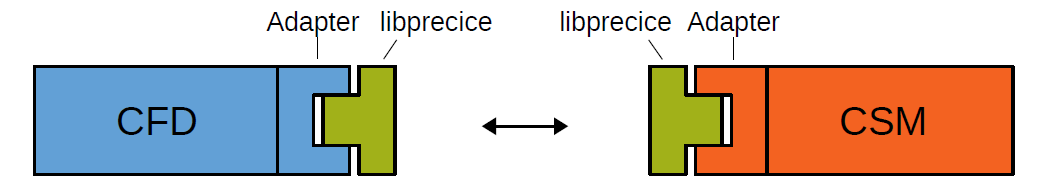
\includegraphics[width=0.92\textwidth]{images/adapter_scheme}
	\caption{Coupling CFD to CSM via preCICE.The existing solver code, the adapter and the linked library are highlighted (image taken from \cite{uekermann2017official}).}
	\label{fig:adapter-scheme}
\end{figure}


\section{Design of the adapter structure}


In order to couple MBDyn with preCICE a C++ adapter has been implemented within the scope of this work. The \textit{adapter} needs to be integrated with both the MBDyn solver and the coupling library. The two connections are distinct but strictly interconnected.
The adapter has the advantage of being completely independent from both the preCICE library and MBDyn. The first connection is achieved via the API given by the library \texttt{libprecice.so}, the second connection exploits the API given by MBDyn through its library \texttt{libmbc.so}.


\section{Structure of the code}

The code for the adapter is available through a public git repository\footnote{\href{https://gitlab.com/Ccaccia73/mbdyn-adapter-test/-/tree/develop}{mbdyn-beam-adapter}}. The code is conceptually divided in two classes, as illustrated in Figure \ref{fig:adapter-classdiag}.

The main class is \texttt{MBDynAdapter}, which implements the functions given by the preCICE interface. It has access to the class \texttt{MBDynConnector} which takes care of all the aspects regarding MBDyn. Attributes, methods and operations of each class are briefly described in the following sections.

\begin{figure}[htbp!]
	\centering
	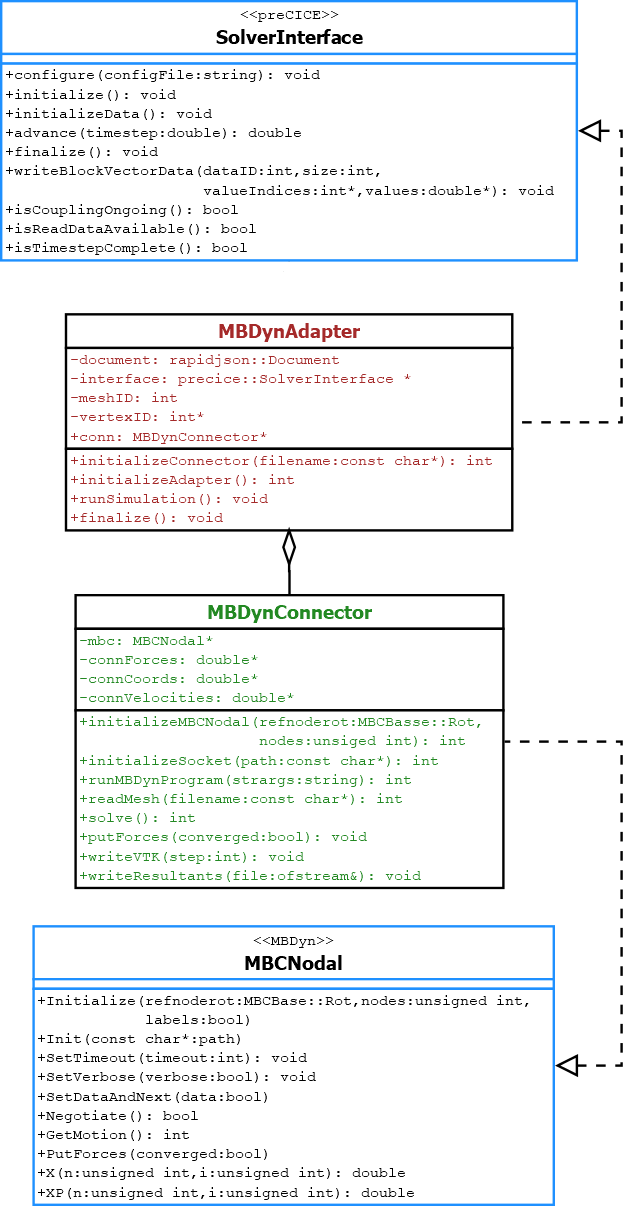
\includegraphics[width=0.8\textwidth]{images/classdiag2}
	\caption{MBDyn adapter class structure}
	\label{fig:adapter-classdiag}
\end{figure}


\subsection{Class MBDynAdapter}
\label{sec:mbdyn-adapter.h}

The file \texttt{MBDynAdapter.h} and its source file \texttt{MBDynAdapter.cpp} implements all the methods required to perform and FSI simulation with MBDyn as the solid solver. The basic steps are:

\begin{enumerate}
	\item prepare the MBDyn solver,
	\item prepare the interface,
	\item provide access to the mesh and initialize the coupling data,
	\item steer the coupled simulation,
	\item finalize the simulation.
\end{enumerate}

\subsubsection{Initialization}

In the initialization phase, the instance of \texttt{MBDynAdapter} gets a \texttt{json} file (see Section \ref{sec:mbdyn-adapter-input}) that contains all the parameters useful for the simulation.
Then it instantiates the \texttt{MBDynConnector} (see Section \ref{sec:mbdyn-connector.h}) which takes care of all the operations concerning MBDyn: in particular starting the simulation the creating an instance of \texttt{MBCNodal} in order to have access to the simulation.

In the next step an instance of \texttt{precice::SolverInterface} is initialized and configured with all the relevant information data:

\begin{itemize}
	\item preCICE configuration file (see Section \ref{sec:pc-config} and Appendix \ref{app:pc-config-file}).
	\item \textit{participant} (i.e. solver) name
	\item information regarding the data to be read and written
\end{itemize} 

The next initialization step concerns the definition of the interface mesh. The data concerning the vertices is stored in the \texttt{MBDynConnector} to be used to plot the output and is passed to the \texttt{SolverInterface} to define the wet surface nodes. The mesh nodes are stored in the same text file that is used by MBDyn to build the \texttt{external structural mapping} information (see Section \ref{sec:mbd-forces}). This means that the MBDyn mapped points coincide with the interface mesh on the structural side (note that it doesn't have to be the same mesh of the fluid side, as preCICE can map non identical meshes, as described in \ref{sec:pc-map}). The suitable size of memory is then initialized to contain the coupling information: mainly \textit{displacements}, to be written on the preCICE interface, and \textit{forces}, to be read from the interface.


\subsubsection{Execution}




\subsubsection{Finalization}

In the finalization phase all the object used during the simulation are closed and memory released.



\subsection{Class MBDynConnector}
\label{sec:mbdyn-connector.h}

- mbdynConnector: connection to MBDyn



\section{Input parameters}
\label{sec:mbdyn-adapter-input}

input: json config file

- simulation parameters

\section{Output results}

output: VTK and resultants





%In order to couple SU2 with preCICE, a C++ adapter class named Precice1 is developed in the scope of
%this work. A header file precice.hpp and a source file precice.cpp are the practical outcome. The Precice
%class encapsulates all coupling related activities and separates them from the original SU2 source code.
%It makes use of the high-level API provided by preCICE. Since the adapter is integrated into the source
%code of SU2, it is completely compiled with it (for a description on how to install SU2 with preCICE,
%see Appendix B). This way, coupling is achieved with minimally invasive code changes in SU2 and an
%adaption of the original code is, thus, possible with only small effort, basically reduced to copy-paste
%tasks. The adapter allows for usage of both explicit and implicit coupling strategies implemented in
%preCICE and fully conforms with intra- and interfield parallelism. Moreover, usage of the adapter is
%assimilated to the regular configuration process of SU2, thus, it is embedded smoothly into the software
%suite. All options concerning the usage of preCICE (e.g. switching it on or off, specifying name and
%location of the preCICE configuration file, etc.) are set via the SU2 configuration file. Consequently, no
%recompilation of SU2 is necessary when the user decides to use/not to use preCICE. In addition, a single
%executable, SU2_CFD, is enough to account for single-physics simulations (without preCICE) as well as
%for FSI computations via preCICE. Figure 5.1 shows a schematic representation of the code coupling
%approach.
%Concerning notation of code shown in this chapter (and in the corresponding referenced sections of the
%appendix), it is important to state that SU2 uses several "containers" for storing information (technically,
%they are multiple pointers). E.g. a "config_container” is an instance of CConfig or a "geometry_container"
%refers to CGeometry. Furthermore, all shown code excerpts are reduced to the necessary information.
%Therefore, not all arguments of functions are stated but only the relevant ones. Also, ellipses (...) are
%used to denote further lines of code, which are not shown for the sake of simplicity.
%This chapter is organized in the following top-down way: Starting from the most user-respective changes
%in SU2, in Section 5.1, the newly added, coupling-related options included in the SU2 configuration
%file are presented and their usage is explained. In addition, necessary code changes are stated. The
%chapter continues with a more technical, detailed description on how the coupling is embedded in SU2,
%as in Section 5.2 adaptions to the main routine of SU2_CFD are described. Mostly, these modifications
%include calling several functions, which are incorporated in the adapter class Precice. However, the tasks
%hidden in these functions are not described until finally, the adapter itself is extensively explained with
%emphasis on both physical and computational details at the end of this chapter in Section 5.3. Referring
%back to Figure 5.1, Sections 5.1 and 5.2 correspond to "code changes" in SU2, while Section 5.3 relates
%to the "Coupling Adapter".
%5.1 Changes Concerning SU2 Configuration
%In order to fully control the usage of preCICE for FSI simulations within SU2, new options in the
%configuration file of SU2 are available (for a recapitulation of this file, see Section 4.2.2). They are listed
%in the following with their default values:
%PRECICE_USAGE = NO, YES (5.1a)
%PRECICE_CONFIG_FILENAME = precice.xml (5.1b)
%PRECICE_VERBOSITYLEVEL_HIGH = NO, YES (5.1c)
%PRECICE_WETSURFACE_MARKER_NAME = wetSurface (5.1d)
%Most obvious, PRECICE_USAGE is a flag used for determining whether a simulation should be run
%with or without preCICE. Modifying the remaining three options is only reasonable if it is set to YES.
%PRECICE_CONFIG_FILENAME specifies the name of the configuration file of preCICE. Also, its path
%relative to the location of the SU2 configuration file must be specified. In order to allow users to have more
%insight into the sequence of activities within the coupling adapter, the level of verbosity of the adapter can
%be chosen. If PRECICE_VERBOSITYLEVEL_HIGH is set to YES, several checkpointing information
%of the adapter is output to the console. Yet, too much console output can slow down simulations. Since
%this information is typically not relevant when running an FSI simulation productively, the verbosity level
%is chosen to be low by default. This feature of the coupling adapter is mainly included for tracing back
%runtime errors. Eventually, as explained in Section 4.2.2, physical boundaries are treated as markers in
%SU2. Each boundary has a unique identifying name, which is specified in the SU2 mesh file. The boundary
%marker name corresponding to the FSI interface of the fluid mesh must be passed to the coupling adapter,
%which is done via the option PRECICE_WETSURFACE_MARKER_NAME. A description on how to
%adapt SU2 in order to use the new configuration options is given in Listings A.1, A.2 and A.3, Appendix
%A to a detailed level.
%The dynamic mesh capabilities of SU2 must be enabled, in order to use the implemented ALE formulation
%of the flow solver. This is done via:
%GRID_MOVEMENT = YES (5.2)
%Still, a specific kind of grid movement needs to be chosen. Intrinsically available are e.g. specifications
%for rigid motions or rotations of the mesh. Here, a new option is available, which is mandatory if SU2 is
%used for FSI simulations via preCICE:
%GRID_MOVEMENT_KIND = PRECICE_MOVEMENT (5.3)
%A manual on how to add this new grid movement option to the configuration procedure of SU2 is given
%in Listing A.4, Appendix A.
%Yet, the implementation of PRECICE_MOVEMENT is missing. It defines the steps of which the mesh
%movement procedure consists. After displacements of the nodes at the wet surface are transferred to
%SU2 via preCICE, the mesh needs to be deformed and smoothed (for a reminder, see Sections 2.2.3 and
%3.3). Despite the sole mesh deformation, also grid velocities must be calculated in order to be able to
%use the ALE method of SU2. Finally, for cases in which the SU2 multigrid capabilities are enabled,
%displacements and velocities of the mesh nodes need to be mapped to all grid levels. Intrinsic SU2
%mesh movement procedures cannot be reused as either they do not include the three necessary steps
%stated above (mesh deformation, grid velocity computation, forwarding information to multigrid levels)
%or they involve further computations, which are not necessary for FSI simulations and therefore, represent
%unnecessary computation overhead. The code defining the steps of PRECICE_MOVEMENT is given in
%Listing A.5, Appendix A.
%
%5.2 Adaption of SU2 Main Routine
%After modifying files related to the configuration procedure of SU2 in the previous section, it remains to
%adapt the SU2_CFD module in SU2_CFD.cpp, which relates to the solver run procedure itself. The goal
%is to add as little code as possible in the main solver routine of SU2 such that the coupling adapter can
%be used. Detailed, corresponding code excerpts are stated in Appendix A.
%One core criterion for integrating the adapter into SU2 is that the solver executable should be able
%to run both single- and multiphysics simulations without recompilation. Only a single adapter-related
%variable needs to be initialized in the main routine of SU2 regardless of whether preCICE is used for a
%simulation or not. The variable (called precice_usage) is a boolean flag corresponding to the newly added
%PRECICE_USAGE option of the SU2 configuration file. This flag is the basis for conditionally triggering
%all coupling activities. If it is set to false, no more coupling variables are initialized in SU2_CFD and
%the single-physics solver runs according to the regular scheme previously shown in Algorithm 2, Section
%4.2.2. The (only three) additional variables needed for coupling include an instance of the adapter class
%Precice and two time-stepping variables (namely max_precice_dt and dt).
%preCICE needs to be able to shut down SU2, in case the FSI simulation should be ended. Therefore, an
%adaption of the main solver while-loop is necessary. In case a simulation runs without preCICE, the usual
%condition of the while-loop is used, which checks that the number of solver iterations is smaller than a
%specified maximum. However, if a coupled FSI simulation is executed, the adapter additionally evaluates
%if preCICE signalizes a solver shut down.
%Assuming that the solver loop is executed, a checkpointing procedure for implicit coupling strategies of
%preCICE starts. For strongly coupled algorithms, preCICE tries to find the fixed-point of the coupling
%equation system (as explained in Section 4.1.1). If the solution of a subiteration does not satisfy the pre-
%CICE convergence criteria, resetting the fluid solver to the start of the time step is necessary. Therefore,
%at the beginning of each solver iteration in SU2, the current solver state is saved such that reloading it
%becomes possible. However, this is only done in the first subiteration of a new time step.
%As mentioned in Section 4.1, preCICE might need to enforce time step sizes for the single-physics solvers.
%To allow for the same in SU2, the minimally allowed time step size for an iteration needs to be determined
%before the solution procedure starts. Here, the variables dt and max_precice_dt come into play. While
%the former stores the current time increment of SU2, the latter is the maximum prescribed by preCICE.
%After SU2 is done with executing a single solver iteration, preCICE is informed that a new flow solution
%is available. Therefore, the coupling tool might advance in time. This triggers preCICE to manage the
%data exchange between SU2 and other coupled solvers, as well as to execute the coupling algorithm. In
%case of an implicit procedure, convergence acceleration techniques are also activated by this step.
%In case a strongly coupled algorithm is chosen, preCICE needs to evaluate (by checking its convergence
%criteria) whether the old solver state of SU2 needs to be reloaded, staying at the same physical time
%instance, or the simulation can proceed with the next time step. In the former case, SU2 internal solver
%variables are reset to the last time instance. It is not reasonable to allow SU2 to write output files if
%preCICE signalizes that the current time step has not sufficiently converged.
%Finally, SU2_CFD handles the clean shut down procedure at the end of an FSI simulation. Communication
%channels are closed via the adapter and coupling-related memory is deallocated.
%In Appendix A the extended solver procedure of SU2_CFD is depicted in Algorithm 4 by analogy with
%the original solver sequence shown in Algorithm 2.
%
%5.3 Coupling Adapter
%As shown in the previous section, most code changes in SU2_CFD consist of conditional clauses checking
%whether the adapter is used, followed by function calls on the adapter object. In this section I explain
%the adapter functions and how they relate to preCICE. No code excerpts are included in this section, as
%the files precice.hpp and precice.cpp will soon be included in the open-source preCICE repository. Thus,
%the interested reader is referred to the source code.
%The adapter makes use of the high-level API provided by preCICE. Its main component is an interface
%with predefined functions that need to be integrated in the adapter. The corresponding class (in preCICE)
%is called SolverInterface. Simply calling functions of this class within SU2 is not sufficient for coupling.
%Rather, the adapter also takes care of
% force calculation at the FSI interface,
% managing intrafield parallelization of SU2 in the coupling process,
% converting data from SU2 to preCICE specific representation and vice versa,
% setting up and triggering mesh deformation,
% as well as reading and writing iteration checkpoints.
%All these functionalities are smoothly hidden within the adapter class. Directly integrating these tasks in
%SU2 would imply highly invasive code changes in its main routines. Yet, the adapter class also contains
%some functions, which I refer to as wrappers. They consist of not much more but function calls on
%SolverInterface. The advantage of this technique is obvious: There is no need to instantiate an object of
%class SolverInterface directly in SU2. Rather, only the adapter instantiates such an object and therefore
%hides it from the main solver routines. Table 5.1 gives an overview of functions2 of the adapter class
%Precice and whether they are wrappers or not.
%function name wrapper function?
%configure() yes
%initialize() no
%advance() no
%isCouplingOngoing() yes
%isActionRequired() yes
%getCowic() no
%getCoric() no
%saveOldState() no
%reloadOldState() no
%finalize() yes
%Table 5.1: Functions of the adapter class Precice and their characterization.
%Some aspects of the adapter functions are already mentioned in Section 5.2. However, detailed explanations
%of what these functions do and their connection to preCICE is eventually given in the following.
%
%Startup of a Coupled Simulation
%The whole coupling process starts with the instantiation of the adapter within the main solver routine of
%SU2. Upon creation of the adapter object, several information is passed to it, including MPI rank and
%size, as well as all geometry (CGeometry), solver (CSolver), configuration (CConfig) and grid movement
%(CVolumetricMovement) related data. Next to initializing data structures needed for coupling, the most
%important step is the instantiation of a SolverInterface object within the adapter, which represents the
%adapter’s connection to preCICE (compare Figure 5.1).
%The adapter object and its connection to preCICE are established, yet it still remains to configure
%preCICE from its configuration file. This happens when configure() is called on the adapter with the
%name and location of the configuration file as input argument. Since this function is a wrapper, internally
%the adapter calls the same function on SolverInterface and forwards name and location of the .xml file.
%Consequently, preCICE parses the configuration file and creates necessary data structures for coupling.
%Subsequently, communication between SU2 and its coupling partner, as well as preCICE internal meshing
%at the wet surface needs to be initiated, which happens upon calling initialize() on the adapter. It checks
%each node at the FSI interface and stores its coordinates in a data array, which is then forwarded to
%preCICE via the SolverInterface object. It is important to keep in mind that intrafield parallelism is
%possible in SU2. The corresponding domain decomposition procedure (for a recapitulation, see Section
%4.2.3) can lead to situations, in which a process does not work on the wet surface at all. This is taken into
%account in the adapter as follows: As mentioned in Section 5.1, the boundary marker name of the wet
%surface must be given to SU2 during configuration. This name is now used to determine whether a process
%includes FSI interface nodes or not. Consequently, the respective process is marked by a boolean flag,
%processWorkingOnWetSurface. If it evaluates to false, the before mentioned coordinate transfer procedure
%is skipped. After receiving the node coordinate information, preCICE is prepared to create an interface
%mesh from it. Finally, initialize() is executed on the SolverInterface object, which triggers setting up
%communication between the coupling partners, creating the wet surface mesh and computing a possible
%restriction on the first time step of SU2.
%
%Coupling Step
%The actual coupling activities start with the main solver loop of SU2. As explained in Section 5.2, a solver
%iteration only occurs if preCICE signalizes that the coupling should not be stopped yet. Therefore, in the
%wrapper function isCouplingOngoing() a function of the same name is executed on the SolverInterface
%object and its boolean return value serves as the demanded signal. Subsequently, at the beginning of an
%iteration and in case an implicit coupling algorithm is chosen, preCICE needs to inform SU2 whether
%the current iteration corresponds to the first one of a new time step. isActionRequired() is called on
%the adapter, which is again just a wrapper for the same function call on SolverInterface. The input
%argument, however, specifies whether the action refers to writing or reading an iteration checkpoint. For
%this purpose, the adapter includes two constant string member variables. One corresponds to writing
%and one to reading a checkpoint. They can be accessed by the respective getter-functions getCowic()
%and getCoric(). In this case, the former is chosen since the adapter might have to write an iteration
%checkpoint.
%If so, saveOldState() is called on the adapter. The goal of saving the current ("old") solver state is to
%store all information, which is necessary to be able to rerun exact the same iteration, implying that an
%iteration of SU2 with the same computational outcome is expected, if the input is not changed. This is
%important for implicit coupling algorithms of preCICE if convergence is not met and a time step needs
%to be restarted. Then, preCICE varies the input of SU2 in terms of the transferred displacements, which
%might yield a better result (in terms of forces), meaning that the residuals of the coupled fixed-point
%system are reduced. The quantities, which need to be stored for this checkpointing strategy, include
%variables associated with the nodal coordinates of the fluid mesh, the grid movement and the solution of
%previous time steps.
%After a solver iteration of SU2 advance() is called on the adapter object. This function is the adapter’s
%most extensive one as it includes computing forces at the wet surface and transferring them to preCICE.
%Moreover, it triggers the coupling algorithm in preCICE, as well as receiving and setting the nodal
%displacements at the FSI interface computed by the structural solver. There is no predefined function
%available in SU2, which computes forces at certain mesh nodes. Therefore, I implemented this computation
%in the advance() function. First of all, the adapter again checks whether the respective MPI process works
%on the wet surface or not via processWorkingOnWetSurface. Computing and forwarding forces is only
%necessary for the nodes in immediate contact with the FSI interface. If a process includes wet surface
%nodes, the adapter determines the kind of flow regime of SU2 (compressible or incompressible, viscous or
%inviscid flow). As mentioned in Section 4.2.1, SU2 is currently not able to run incompressible simulations
%with ALE support. However, I already include the force computation for incompressible flows in the
%adapter, in case this capability will be added in future releases. In addition, the adapter computes a
%factor for redimensionalizing forces (as SU2 features non-dimensionalized simulations as well). If the
%current simulation is dimensional, this factor evaluates to 1. In order to explain the force calculation, I
%assume the general, three-dimensional case of a simulation governed by the NSE. The overall force at a
%node acting on the FSI interface is then given by a viscous term arising from the viscous stress tensor
%
%and an inviscid term determined by the (dynamic) pressure. The computation is done as follows:
%fi = 􀀀(ptotal 􀀀 pstatic)niA + ijnjA 8i = 1; 2; 3; with (5.4a)
%ij = (
%@vi
%@xj
%+
%@vj
%@xi
%) 􀀀
%2
%3
%
%@vk
%@xk
%ij 8i; j = 1; 2; 3: (5.4b)
%f denotes the force vector, p pressure (total and static, respectively) and  the viscous stress tensor. A
%and n refer to area and unit outward normal vector of the dual mesh element associated with the node, for
%which the force is calculated. Note that the pressure term needs to be negated as by definition pressures
%point inward the fluid control volume, but the pressure force exerted on the solid (i.e. outward the fluid
%control volume) is required. The explanation of the viscous stress tensor in Equation 5.4b is identical to
%Equation 2.6. Again, the adapter needs to manage intrafield parallel execution of SU2. As extensively
%explained in Section 4.2.3, ghost nodes are introduced in SU2 in order to build halo-cells after domain
%decomposition. If decomposition occurs at the wet surface, interface nodes are replicated. Allowing each
%of the replicates and the original nodes to write forces to preCICE would yield unphysical computation
%results, as those nodes share the same mapping to the solid mesh and therefore, forces would accumulate
%at solid nodes. The adapter makes use of the colors assigned to the FSI interface nodes in SU2. This is
%technically done by comparing the MPI rank (= color of the process) with the colors of the wet surface
%nodes. If they do not match, the process works on a duplicate and thus, is not allowed to write forces
%at such a node. The corresponding data array storing all FSI forces is eventually pushed to preCICE by
%calling writeBlockVectorData() on the SolverInterface instance.
%The next step is executing advance() on the SolverInterface object, which uses the length of the current
%solver iteration of SU2 as input and returns the prescribed maximum for the next iteration. Internally,
%preCICE now executes convergence acceleration techniques, if an implicit procedure is chosen and exchanges
%coupling data with the partner solvers.
%In the following, the adapter needs to read the FSI interface nodal displacements calculated by the coupled
%structural solver. Thus, readBlockVectorData() is called on the SolverInterface object. The so obtained
%displacements are set as coordinate variations relative to the nodal positions of the last time step in SU2.
%While writing forces must be restricted to the nodes originally belonging to a process, reading and setting
%displacements needs to be done also for the replicates.
%Although it would be possible to trigger the mesh deformation procedure right away, I decided against
%this strategy as the current time step might have to be restarted and mesh deformation would be unnecessary
%computational overhead in such a case. Thus, it is triggered at the beginning of the next solver
%iteration as shown in Algorithm 3.
%Now the counterpart of writing an iteration checkpoint comes into play (only for implicit algorithms).
%preCICE checks whether the fixed-point equation system converges sufficiently or not. In the latter case,
%upon calling the wrapper function isActionRequired() with input argument getCoric() on the adapter,
%the coupling tool signalizes that reloadOldState() needs to be executed. Consequently, the solver state
%prior to the current iteration is retrieved by resetting the respective variables in SU2.
%
%Clean Exit
%The main solver loop of SU2 is usually exited when isCouplingOngoing() in the while-loop condition
%evaluates to false, which means that preCICE tries to finish the FSI simulation. The last step of the
%coupling is initiated when the wrapper function finalize() is executed on the adapter object. This causes
%all communication channels related to the coupled simulation to be closed and used memory to be
%deallocated.

